\chapter{系統架構與實作}

    本研究所設計之系統系利用超音波對麥克風造成的非線性響應輸出與主動式噪音控制消除高關聯度噪音等特性。
來嘗試解決在部署麥克風干擾器的場域裡無法取得有效聲學紀錄的問題。
同時藉由密碼系統的機密性與不可否認性,發展一套以其為基礎的會談錄音存取控制機制。
透過上述機制的結合,能夠使在部署超音波麥克風干擾器的會談情境中,於會談結束後,允許特定參與者得以取得有效之聲音記錄。


\section{符號定義}

    本研究設計之系統所使用符號與其意義如表 \ref{table:tab.symbol} 所示。

\rowcolors{1}{white}{whitesmoke}
\begin{longtable}{c l}
    \hiderowcolors
    \caption{符號定義表} \label{table:tab.symbol} \\

    \hiderowcolors
    \hline
    \multicolumn{1}{c}{\bf{符號}} & \multicolumn{1}{c}{\bf{釋義}} \\
    \hline
    \endfirsthead

    \hiderowcolors
    \multicolumn{1}{c}{\bf{符號}} & \multicolumn{1}{c}{\bf{釋義}} \\
    \hline
    \endhead

    \hiderowcolors
    \hline
    \endlastfoot

    \showrowcolors
    \DEFattender    & 第 $h$ 位會談參與者 (Attender) \\
    \DEFowner       & 第 $i$ 位會談擁有者 (Owner) \\
    \DEFownerID     & 會談擁有者 $i$ 的唯一識別碼 \\
    \DEFpublicKey   & 會談擁有者 $i$ 的公開金鑰 \\
    \DEFprivateKey  & 會談擁有者 $i$ 的私密金鑰 \\
    \DEFagentKey    & 會談擁有者 $i$ 的代理金鑰 (Agent Key) \\
    \DEFakEnc       & 透過會談擁有者 $i$ 的公開金鑰所加密的 \DEFagentKey \\
    \DEFakEncDec    & 透過會談擁有者 $i$ 的私密金鑰所解密的 \DEFakEnc \\
    \DEFakEncDecSig & \DEFakEncDec 的數位簽章 \\
    \DEFsessionID   & 當次會談唯一識別碼 \\
    \DEFunsealKey   & 當次會談的解封金鑰 (Unseal Key) \\
    \DEFfuncEncEK   & 對稱式加密演算法之加密函數 \\
    \DEFfuncDecEK   & 對稱式加密演算法之解密函數 \\
    \DEFfuncSignSK  & 使用私密金鑰 $sk$ 的數位簽章演算法簽之名函數 \\
    \DEFfuncVerfPK  & 使用公開金鑰 $pk$ 的數位簽章演算法之驗證函數 \\
    \DEFfuncEncPK   & 使用公開金鑰 $pk$ 的非對稱式加密演算法之加密函數 \\
    \DEFfuncDecSK   & 使用私密金鑰 $sk$ 的非對稱式加密演算法之解密函數 \\
    \DEFfuncPRNG    & 偽隨機數產生器演算法函數 \\
    \DEFseed        & 用於當次會談的偽隨機數產生器種子 \\
    \DEFrecJ        & 於開啟音波麥克風干擾器場域裡的會談聲音記錄 \\
    \DEFrecN        & 純超音波麥克風干擾器於麥克風的響應輸出之聲音記錄 \\
    \DEFrecREV      & 執行系統機制 {\it Unseal} 所產生之有效會談聲音記錄 \\
    \DEFtimeMAX     & 會談進行時間長度的最大值、\DEFrecN 的時間長度 \\
    \hiderowcolors
\end{longtable}


\section{系統架構}

\begin{figure}[H]
    \centering
    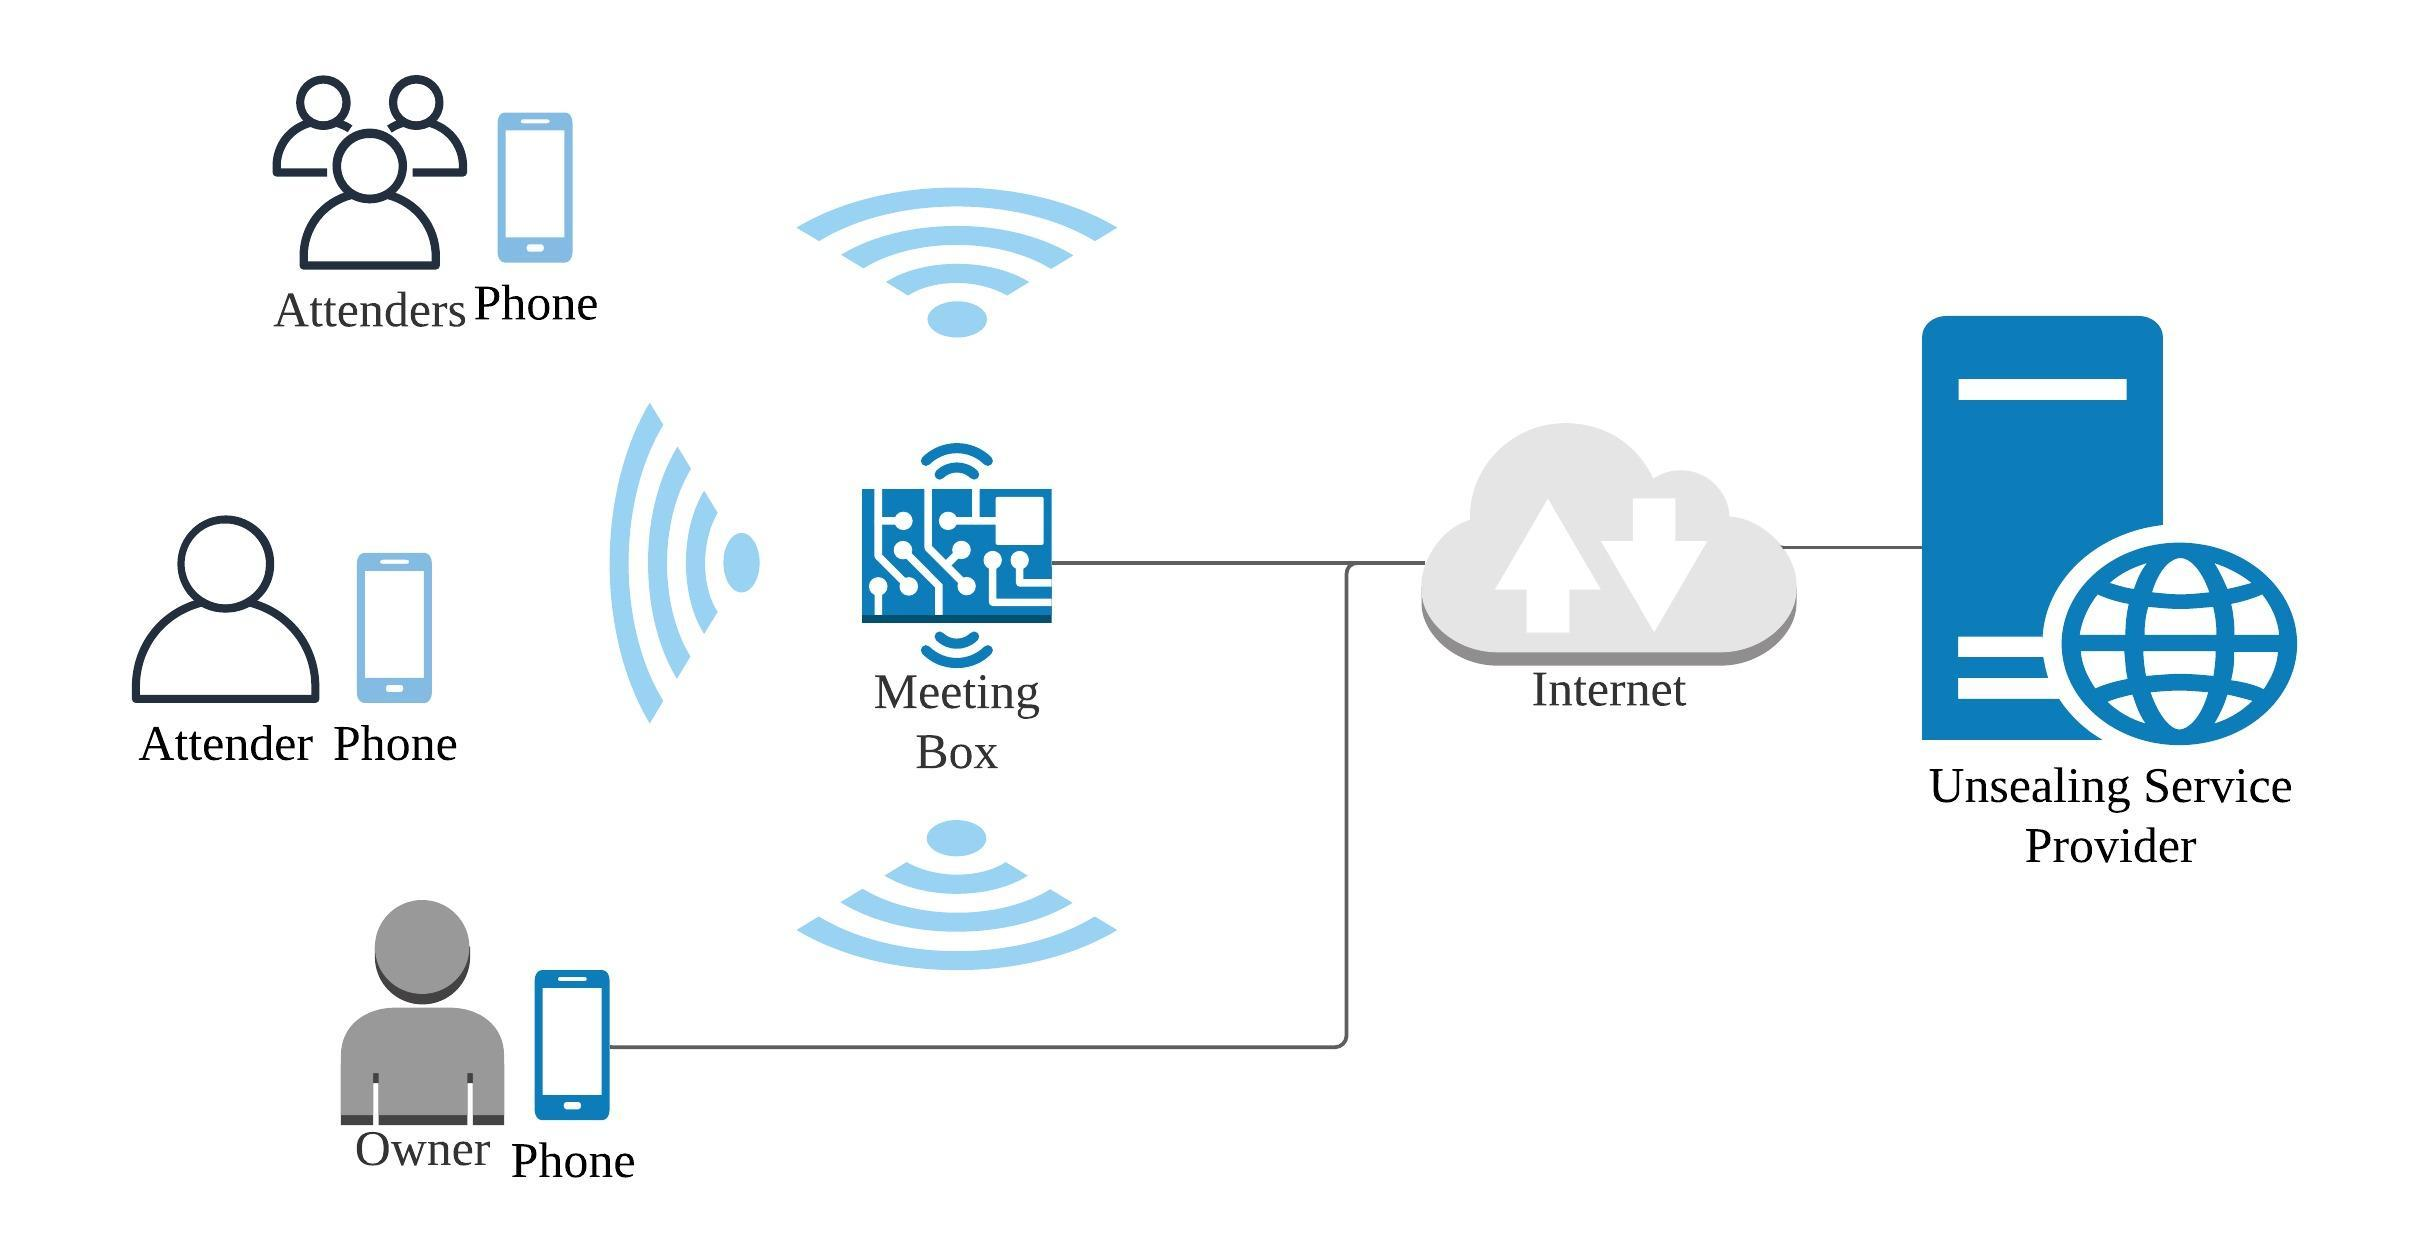
\includegraphics[width=0.8\textwidth]{single-owner-architecture}
    \caption{單一 Owner 系統架構圖}
    \label{fig.s-o-arch}
\end{figure}

    本系統由 MeetingBox、Server 以及會談參與者 Attender 所組成。
各會談的 Attender 僅定義於當次會談,每次參與會談的 Attender 可為不同群體。
Attender 於 MeetingBox 的周圍進行會談 ({\it Meeting Session}),如圖 \ref{fig.s-o-arch}。
MeetingBox 於會談進行間開啟超音波麥克風干擾器,因此鄰近的麥克風或周邊的聲音記錄裝置,
都將因受到其干擾而失效,Attender 無法自行有效記錄會談的聲音內容。

    MeetingBox 於會談進行中持續紀錄聲音,內容為受到超音波麥克風干擾器干擾的會談錄音 (\DEFrecJ)。
於會談結束後,受超音波麥克風干擾器干擾的會談聲音記錄 (\DEFrecJ),
將作為系統機制「解封」({\it Unseal}) 的輸入 (見 \ref{subsec.unseal}),
使會談參與者 Attender 中的會談擁有者 Owner,獲得前述機制所產生的有效會談聲音記錄 (\DEFrecREV)。


\subsection{Attender}

    會談參與者 Attender 為一集合,代表所有當次會談 ({\it Meeting Session}) 的參與者。
Attender 包含 Owner,為 Owner 的超集合。其餘非 Owner 的 Attender 視為 non Owner Attender。
Attender 透過 MeetingBox 上的控制介面與其互動,進而控制系統的生命週期,本研究以實體按鈕為例。

    Attender 受到 MeetingBox 中的超音波麥克風干擾器的干擾,使得隨身的麥克風或聲音記錄裝置,
都將因受到干擾而失效,無法有效記錄會談內容。例如:智慧型手機、智慧手錶、筆電、平板、智慧喇叭等。


\subsection{Owner}

\begin{figure}[H]
    \centering
    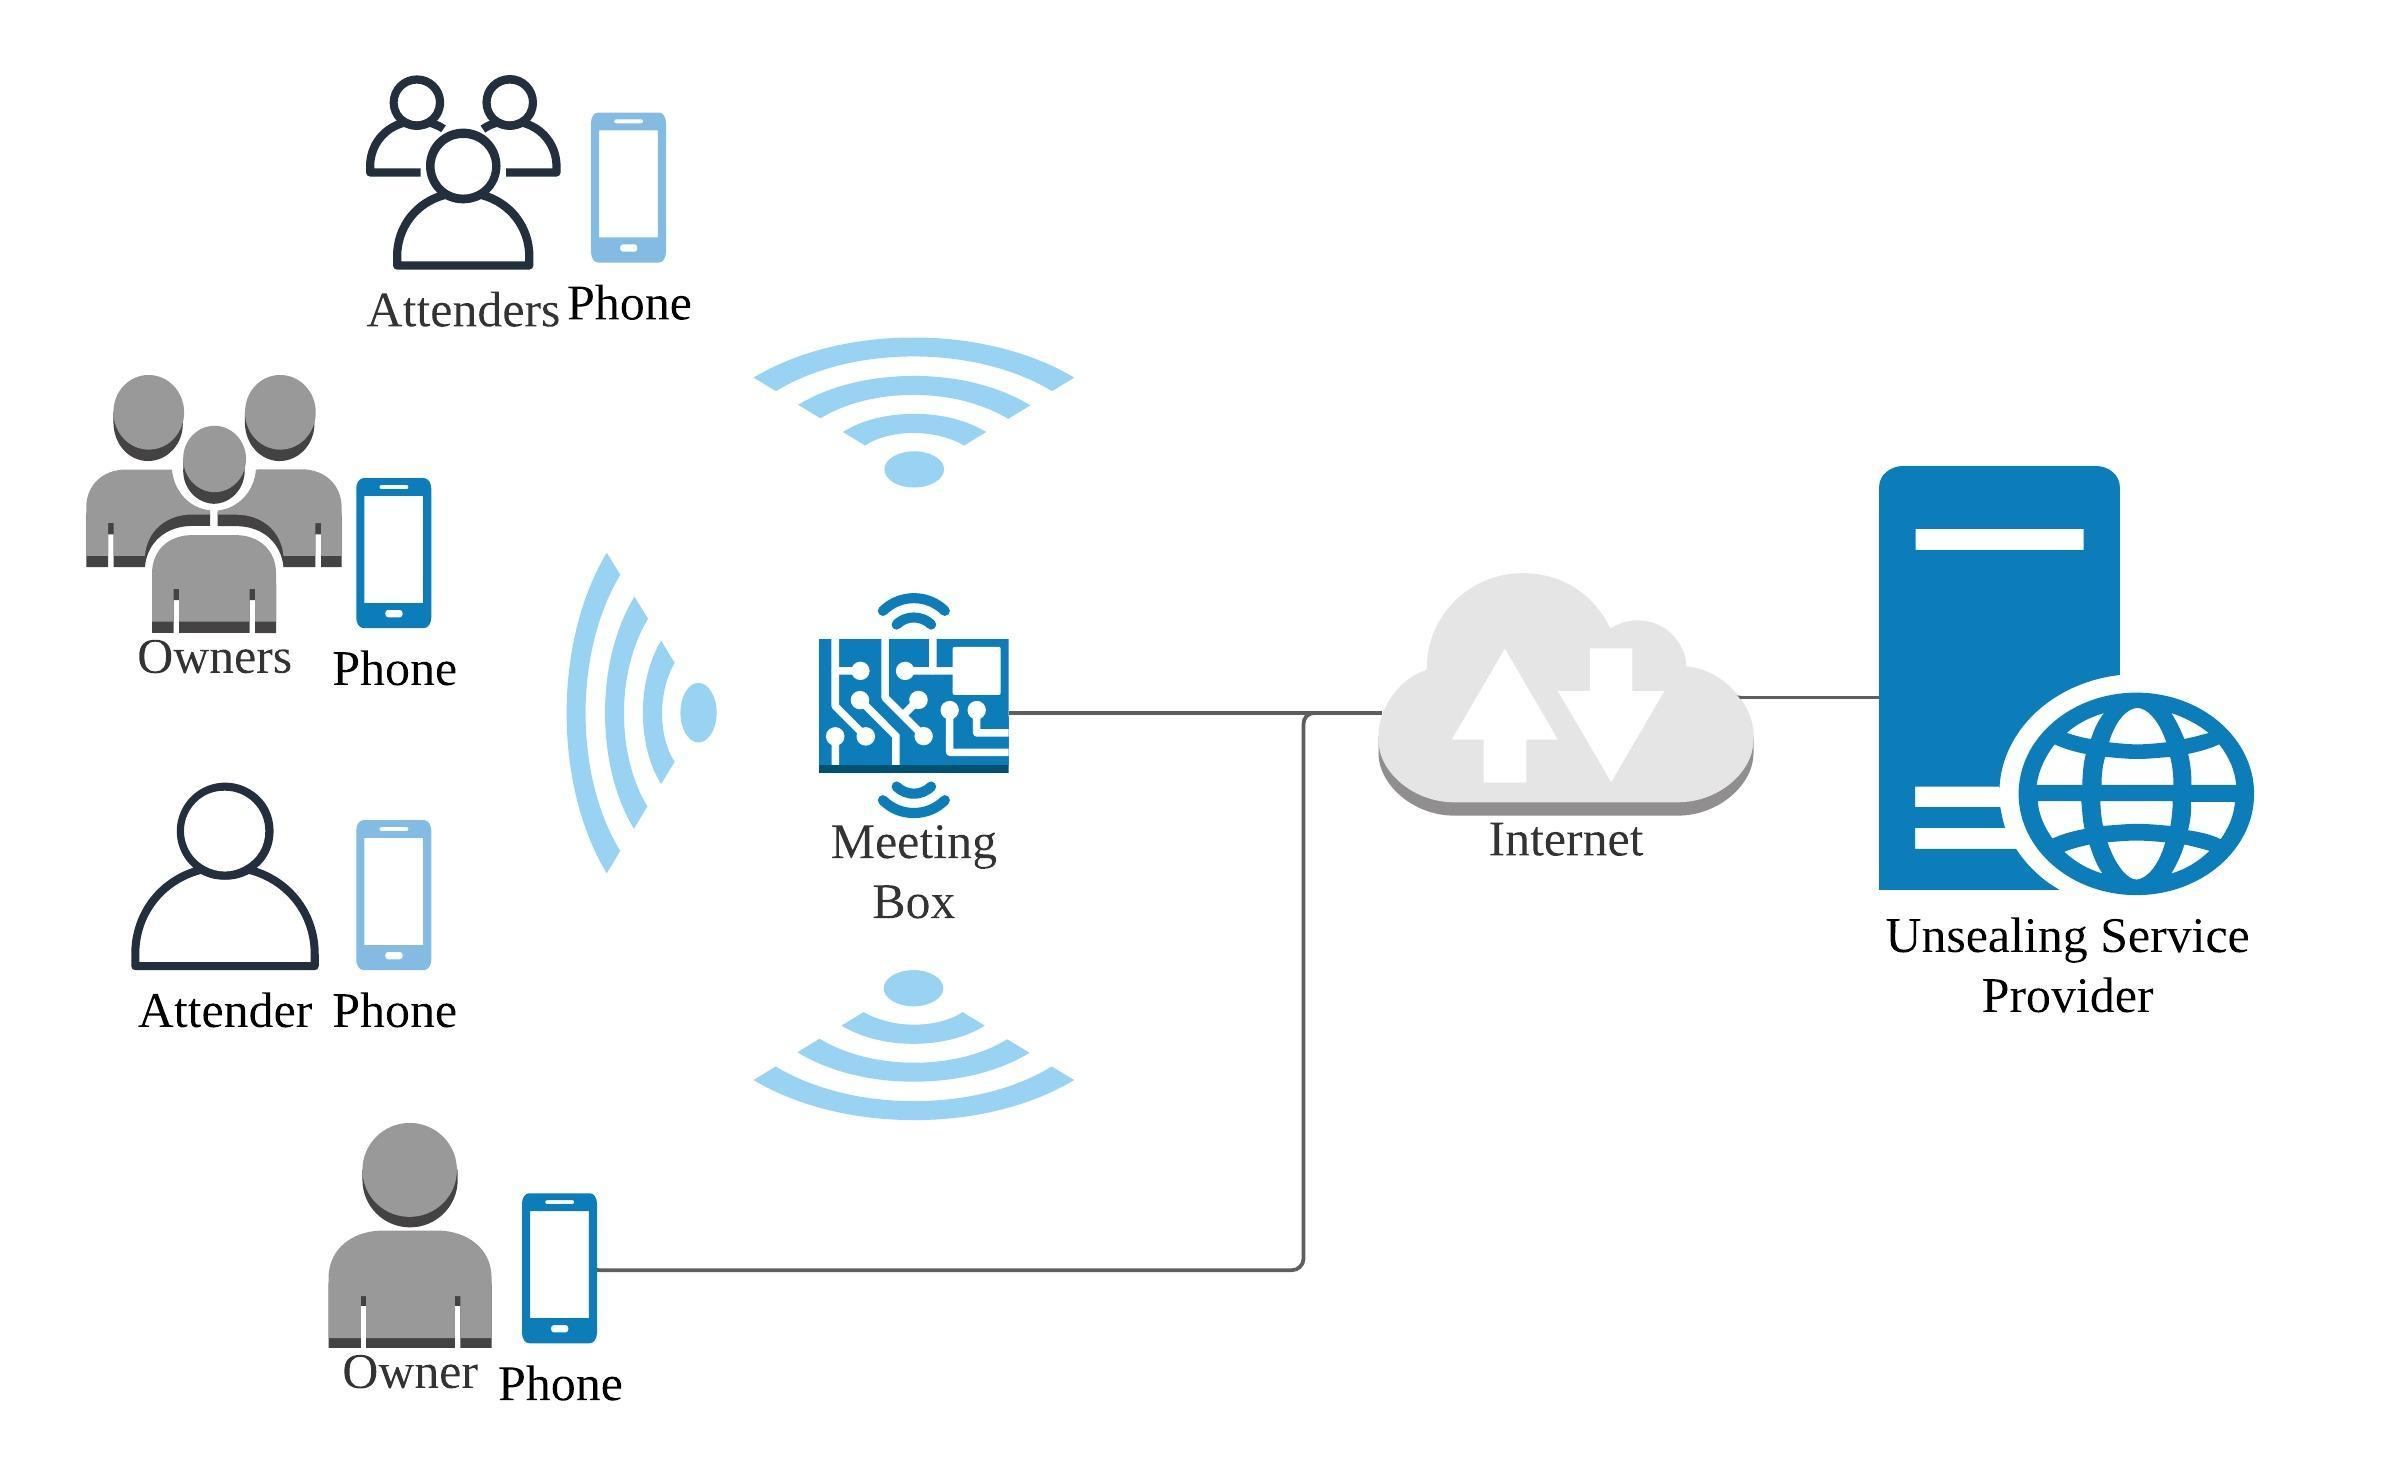
\includegraphics[width=0.8\textwidth]{multi-owner-architecture}
    \caption{多 Owner 系統架構圖}
    \label{fig.m-o-arch}
\end{figure}

    會談擁有者 Owner 屬於 Attender,為 Attender 的子集合,
Owner 定義為 Attender 中的特權角色。Owner 如未執行本研究所設計的系統機制「註冊會談擁有者」 (Register Owner),
則視為 non Owner Attender。 Owner 於會談 ({\it Meeting Session}) 結束後,
有能力決定是否執行系統機制「解封」 ({\it Unseal}),並獲取 {\it Unseal} 所產生的有效會談聲音記錄 (\DEFrecREV)。

    Owner 必須是一或多人。當會談中只有一個 Owner 時,為 {\it Single Owner Meeting Session} 情境,
系統架構如圖 \ref{fig.s-o-arch}。當會談中多於一個 Owner 時,為 {\it Multi Owner Meeting Session} 情境,
系統架構如圖 \ref{fig.m-o-arch} 所示。

    Owner 持有智慧型裝置,透過其與 MeetingBox 互動,獲取 MeetingBox 上的資訊,並有能力於會談進行中、會談結束後,
與 Server 持續通訊,執行本研究所設計的系統機制「註冊會談擁有者」 (Register Owner) 與「解封」 ({\it Unseal})。

    上述 Owner 獲取 MeetingBox 資訊的方法,本研究以掃描 QR Code 為例。


\subsection{MeetingBox}

    MeetingBox 為本研究所設計系統核心組成要件的終端,部署於會談 ({\it Meeting Session}) 的場域,
與會談參與者 Attender 實體接觸。透過與 Attender 的互動,成為觸發會談生命週期改變事件的控制核心。
同時也作為系統聲音紀錄的輸入來源。在本研究的設計中,一組 MeetingBox 僅能同時間處理一場會談的進行。

    本研究所設計的 MeetingBox 裝置包含下列組件:

    \begin{enumerate}
        \item 超音波麥克風干擾器:\\
            使用偽隨機數 \DEFfuncPRNG 產生亂數頻率的超音波,於會談進行中開啟。
            用於干擾鄰近周圍含有麥克風的裝置,使其無法有效記錄會談內容。

        \item 錄音麥克風:\\
            用於紀錄會談的聲音內容 (\DEFrecJ),與產生超音波麥克風干擾器於麥克風的響應輸出 (\DEFrecN)

        \item 物理控制介面:\\
            提供 Attender 操作與 MeetingBox 互動,獲得外部觸發事件。本研究實做以實體按鈕為例。

        \item 人機互動介面:\\
            用於傳遞會談的 meta data 與系統狀態提示給 Attender,本研究實做以 QR Code 搭配螢幕顯示為例。

        \item 運算控制核心與網路介面:\\
            周邊裝置控制與邏輯運算核心,用於加密,與 Server 通訊等運算工作。
    \end{enumerate}


\subsection{Server}

    Server 為本研究所設計的系統核心組成要件之一,其設計能同時間處理一場以上的會談 ({\it Meeting Session}) 的進行,
其角色目標為執行系統機制「解封」 ({\it Unseal})。此機制觸發於會談結束後,Owner 向 Server 發送請求執行。
目的為取得有經系統機制 {\it Unseal} 所產生有效之會談聲音記錄 \DEFrecREV。

    Server 執行系統機制「解封」 ({\it Unseal}) 時,包含以下步驟:
    \begin{enumerate}[itemsep=0pt,parsep=0pt,]
        \item {\it Challenge}: \\
            目標為使 Server 獲得 Owner 授權得以接續執行後續步驟。
        \item 「主動式噪音控制」({\it ANC}): \\
            將受干擾的會談聲音記錄 \DEFrecJ,還原為有效的會談聲音記錄 \DEFrecREV。
    \end{enumerate}


\section{系統流程}

\begin{figure}[H]
    \centering
    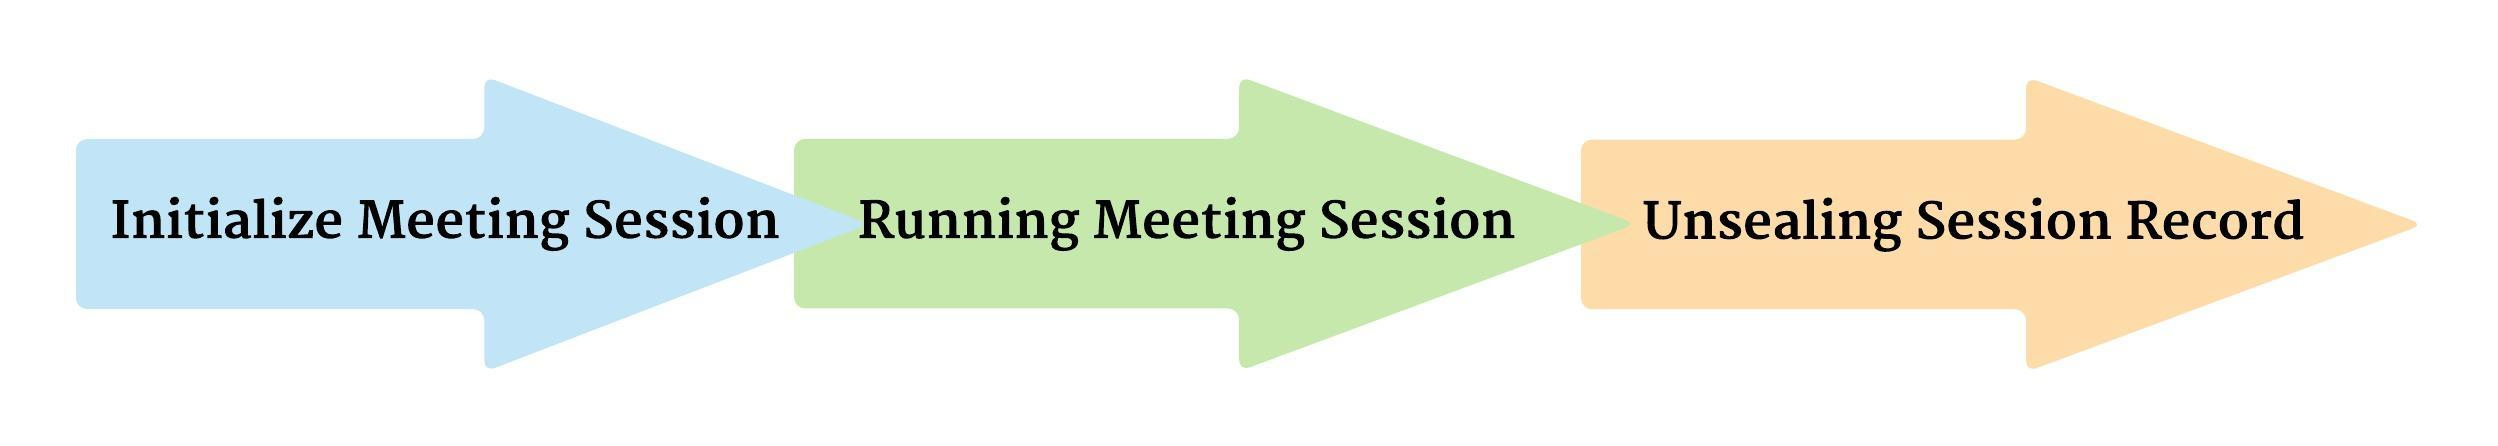
\includegraphics[width=0.9\textwidth]{system-stage}
    \caption{{\it Meeting Session} 生命週期}
    \label{fig.system-stage}
\end{figure}

    本研究所設計之系統,其流程跟隨會談 ({\it Meeting Session}) 的生命週期,其分為三個階段定義。分別為:
一、「初始化會談 (Initialize {\it Meeting Session})」;二、「進行會談 (Running {\it Meeting Session})」;
三、「解封 ({\it Unseal})」;如圖 \ref{fig.system-stage}。

    第一階段作為 {\it Meeting Session} 的起始點,各階段依序執行,於第三階段結束一次系統生命週期的循環。
系統可以同時存在多個{\it Meeting Session}循環,彼此互相互不干擾影響,獨立執行。
本章節將介召個系統生命週期階段的流程步驟,且逐步說明定義系統的關鍵參數。流程步驟將分為兩種情境說明:
一、「{\it Single Owner Meeting Session}」;二、「{\it Multi Owner Meeting Session}」

    MeetingBox 於 {\it Meeting Session} 開始前,已經預先設定時間長度為 \DEFtimeMAX 的 \DEFrecN。
且於第二階段 Running {\it Meeting Session} 中所紀錄的聲音內容之長度,須小於  \DEFtimeMAX。
{\it Meeting Session} 生命週期開始前,MeetingBox 根據此次 {\it Meeting Session} 的 \DEFseed,
預先使用 MeetingBox 內的超音波麥克風干擾器與麥克風,預先錄製產生 \DEFrecN。於 {\it Meeting Session} 結束後,
重新配置與產生 \DEFseed 與 \DEFrecN。


\subsection{初始化會談 (Initialize {\it Meeting Session})}
\label{subsec.initialize}

    此章節將說明 {\it Single Owner Meeting Session} 情境中,
{\it Meeting Session} 生命週期第一個階段:Initialize {\it Meeting Session} 的系統流程。
如圖 \ref{fig.s-o-init} 所示。

\begin{figure}[H]
    \centering
    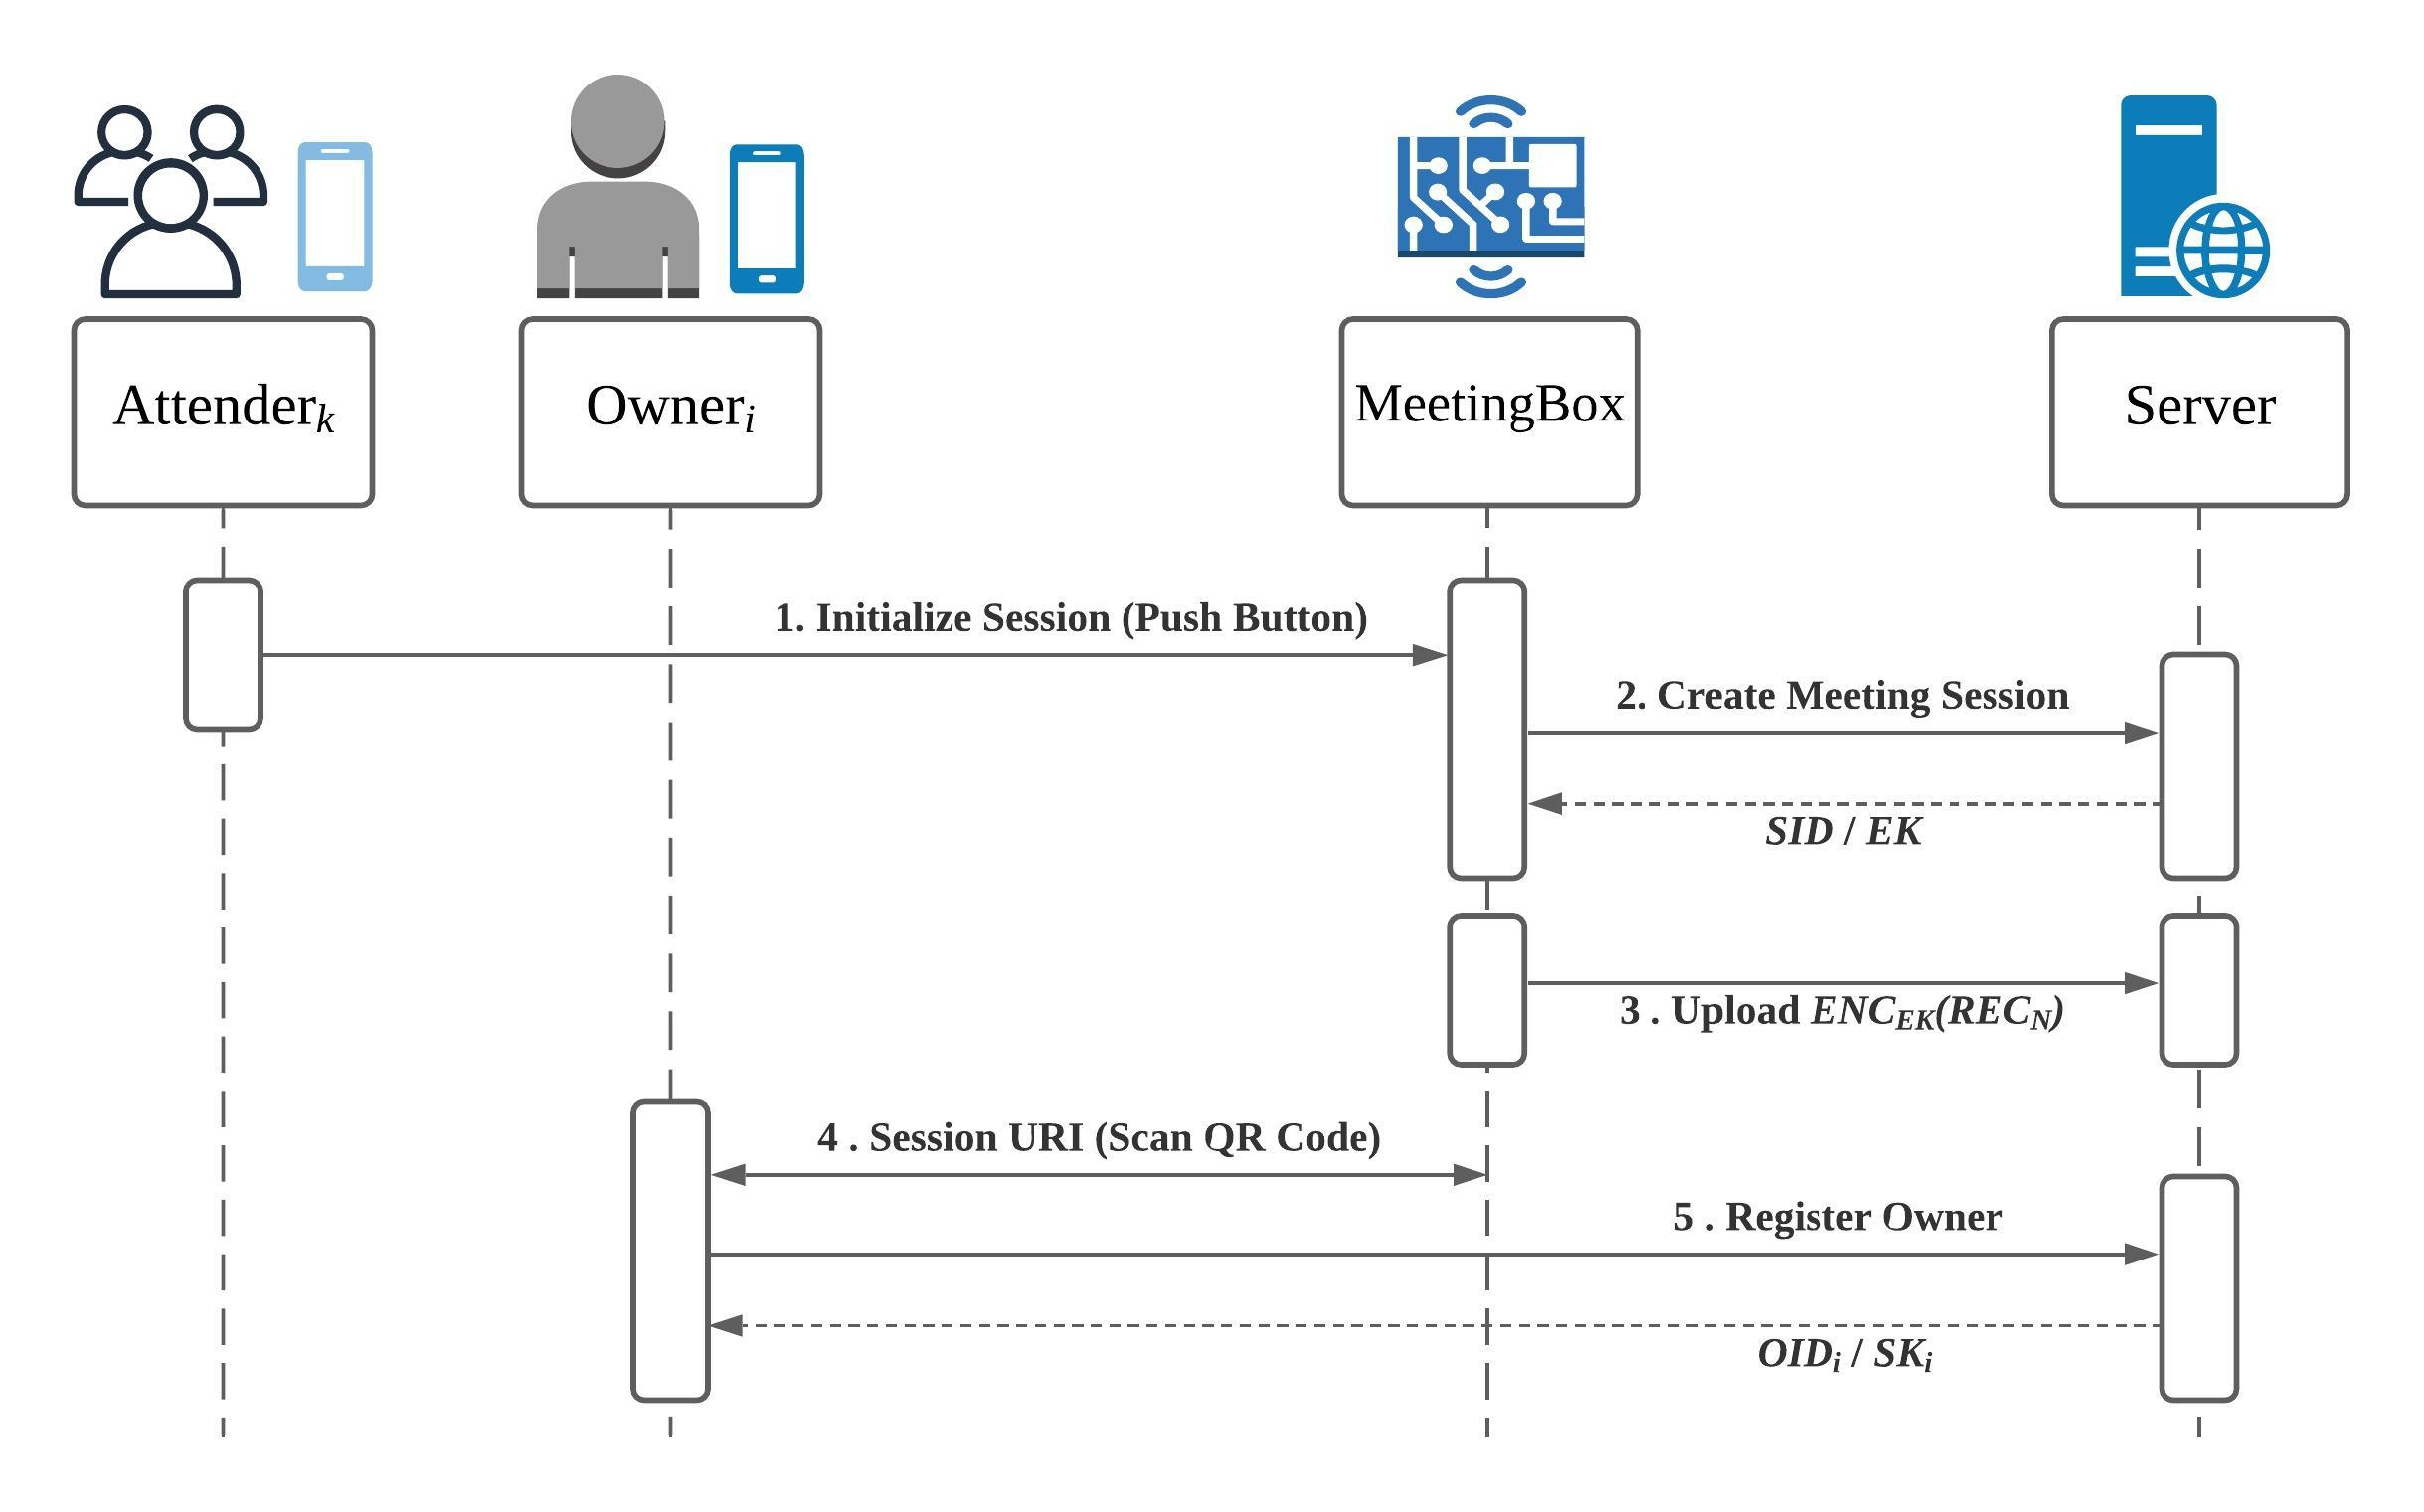
\includegraphics[width=0.9\textwidth]{single-owner-sequence-diagram-init}
    \caption{Single Owner Initialize {\it Meeting Session}}
    \label{fig.s-o-init}
\end{figure}

\begin{steps}
    \item Initialize Session (Push Button):

            Attender 在欲進行會談 MeetingBox 的周圍準備開始會談,\DEFattender 透過 MeetingBox 的物理控制介面,
        使 MeetingBox 獲得外部事件,觸發 Initialize Session。本研究實驗以按鈕為例,
        當 \DEFattender 按下 MeetingBox 上的按鈕後,觸發 MeetingBox 執行 Initialize Session。

    \item Create Meeting Session:

            MeetingBox 觸發 Initialize Session 後,首先對 Server 傳送請求 Create Meeting Session。
        Server 收到請求後產生 (\DEFsessionID, \DEFunsealKey) 並回傳至 MeetingBox。

            其中 \DEFsessionID 為此次 {\it Meeting Session} 的唯一識別碼;\DEFunsealKey 是對稱式加密金鑰,
        定義為此次 {\it Meeting Session} 的解封金鑰 (Unseal Key)。
        \DEFsessionID 的產生必須滿足唯一性,隨機性,不可預測性,本研究實作 \DEFsessionID 以 UUID v4 為例。
        \DEFunsealKey 為對稱式加密的金鑰,其產生方式,本研究所設計之系統以 AES CFB mode 為例。

    \item Upload Encrypted \DEFrecN:

            MeetingBox 收到產生自 Server 的回傳訊息 (\DEFsessionID, \DEFunsealKey)後,使用對稱式加密演算法與金鑰 \DEFunsealKey 加密 \DEFrecN,
        在將加密後的 \DEFrecN 上傳至 Server,並銷毀於 MeetingBox 中的 \DEFunsealKey。

            前述對稱式密鑰演算法,本研究所設計之系統以 AES CFB mode 為例。本文中定義為 \DEFfuncEncEK,
        其輸入為欲加密明文資料,輸出為已加密的密文。

    \item Get Session URI (Scan QR Code):

            MeetingBox 收到產生自 Server 的回傳訊息 (\DEFsessionID, \DEFunsealKey)後,
        將 \DEFsessionID 資訊封裝為此次 {\it Meeting Session} 專用的 URI (Uniform Resource Identifier),
        並傳送給 Owner。URI 的封裝方法為,將 \DEFsessionID 填入系統已知包含 Server 網址的字串。

            前述 MeetingBox 將資訊傳遞給 Owner 的方法,本研究以 MeetingBox 搭配螢幕顯示 QR Code 為例。
        \DEFowner 持智慧裝置,掃描 MeetingBox 螢幕顯示的 QR Code,以獲得 \DEFsessionID 封裝後的 URI 。

    \item Register Owner:

            \DEFowner 收到 MeetingBox 產生的 URI 後,
        使用此 URI 向 Server 進行系統機制「註冊會談擁有者」 (Register Owner)。運作細節如下:
        一、\DEFowner 對 Server 發送 Register Owner 請求;
        二、Server 收到 Register Owner 請求後,隨即產生一組公私金鑰對 (\DEFpublicKey, \DEFprivateKey)
        與 \DEFowner 的唯一識別碼 \DEFownerID,
        並將請求來源 URI 中的 \DEFsessionID 與公開金鑰 \DEFpublicKey 和 \DEFownerID 做關聯綁定;
        三、回傳私密金鑰 \DEFprivateKey 與 \DEFownerID 給 \DEFowner,且銷毀於 Server 中的\DEFprivateKey;

            在 {\it Single Owner Meeting Session} 情境中,只存在一個 Owner,
        因此當唯一 Owner 執行成功後,即完成此系統步驟,進入下一階段。
        Onwer 為 Attender 中的特權角色,其特權來源為 \DEFowner 的 \DEFprivateKey,
        因此 Owner 須妥善保管 \DEFprivateKey,維持其機密性。

            \DEFownerID 的產生必須滿足唯一性,隨機性,
        不可預測性,本研究實作 \DEFownerID 以 UUID v4 為例。
        前述公私金鑰對的產生方法,本研究所設計之系統以 RSA PKCS \#1 為例。
\end{steps}

\subsection{進行會談 (Running {\it Meeting Session})}
\label{subsec.sessioning}

    此章節將說明 {\it Single Owner Meeting Session} 情境中,
{\it Meeting Session} 生命週期第二個階段:Running {\it Meeting Session} 的系統流程。
如圖 \ref{fig.s-o-sessioning} 所示。

\begin{figure}[H]
    \centering
    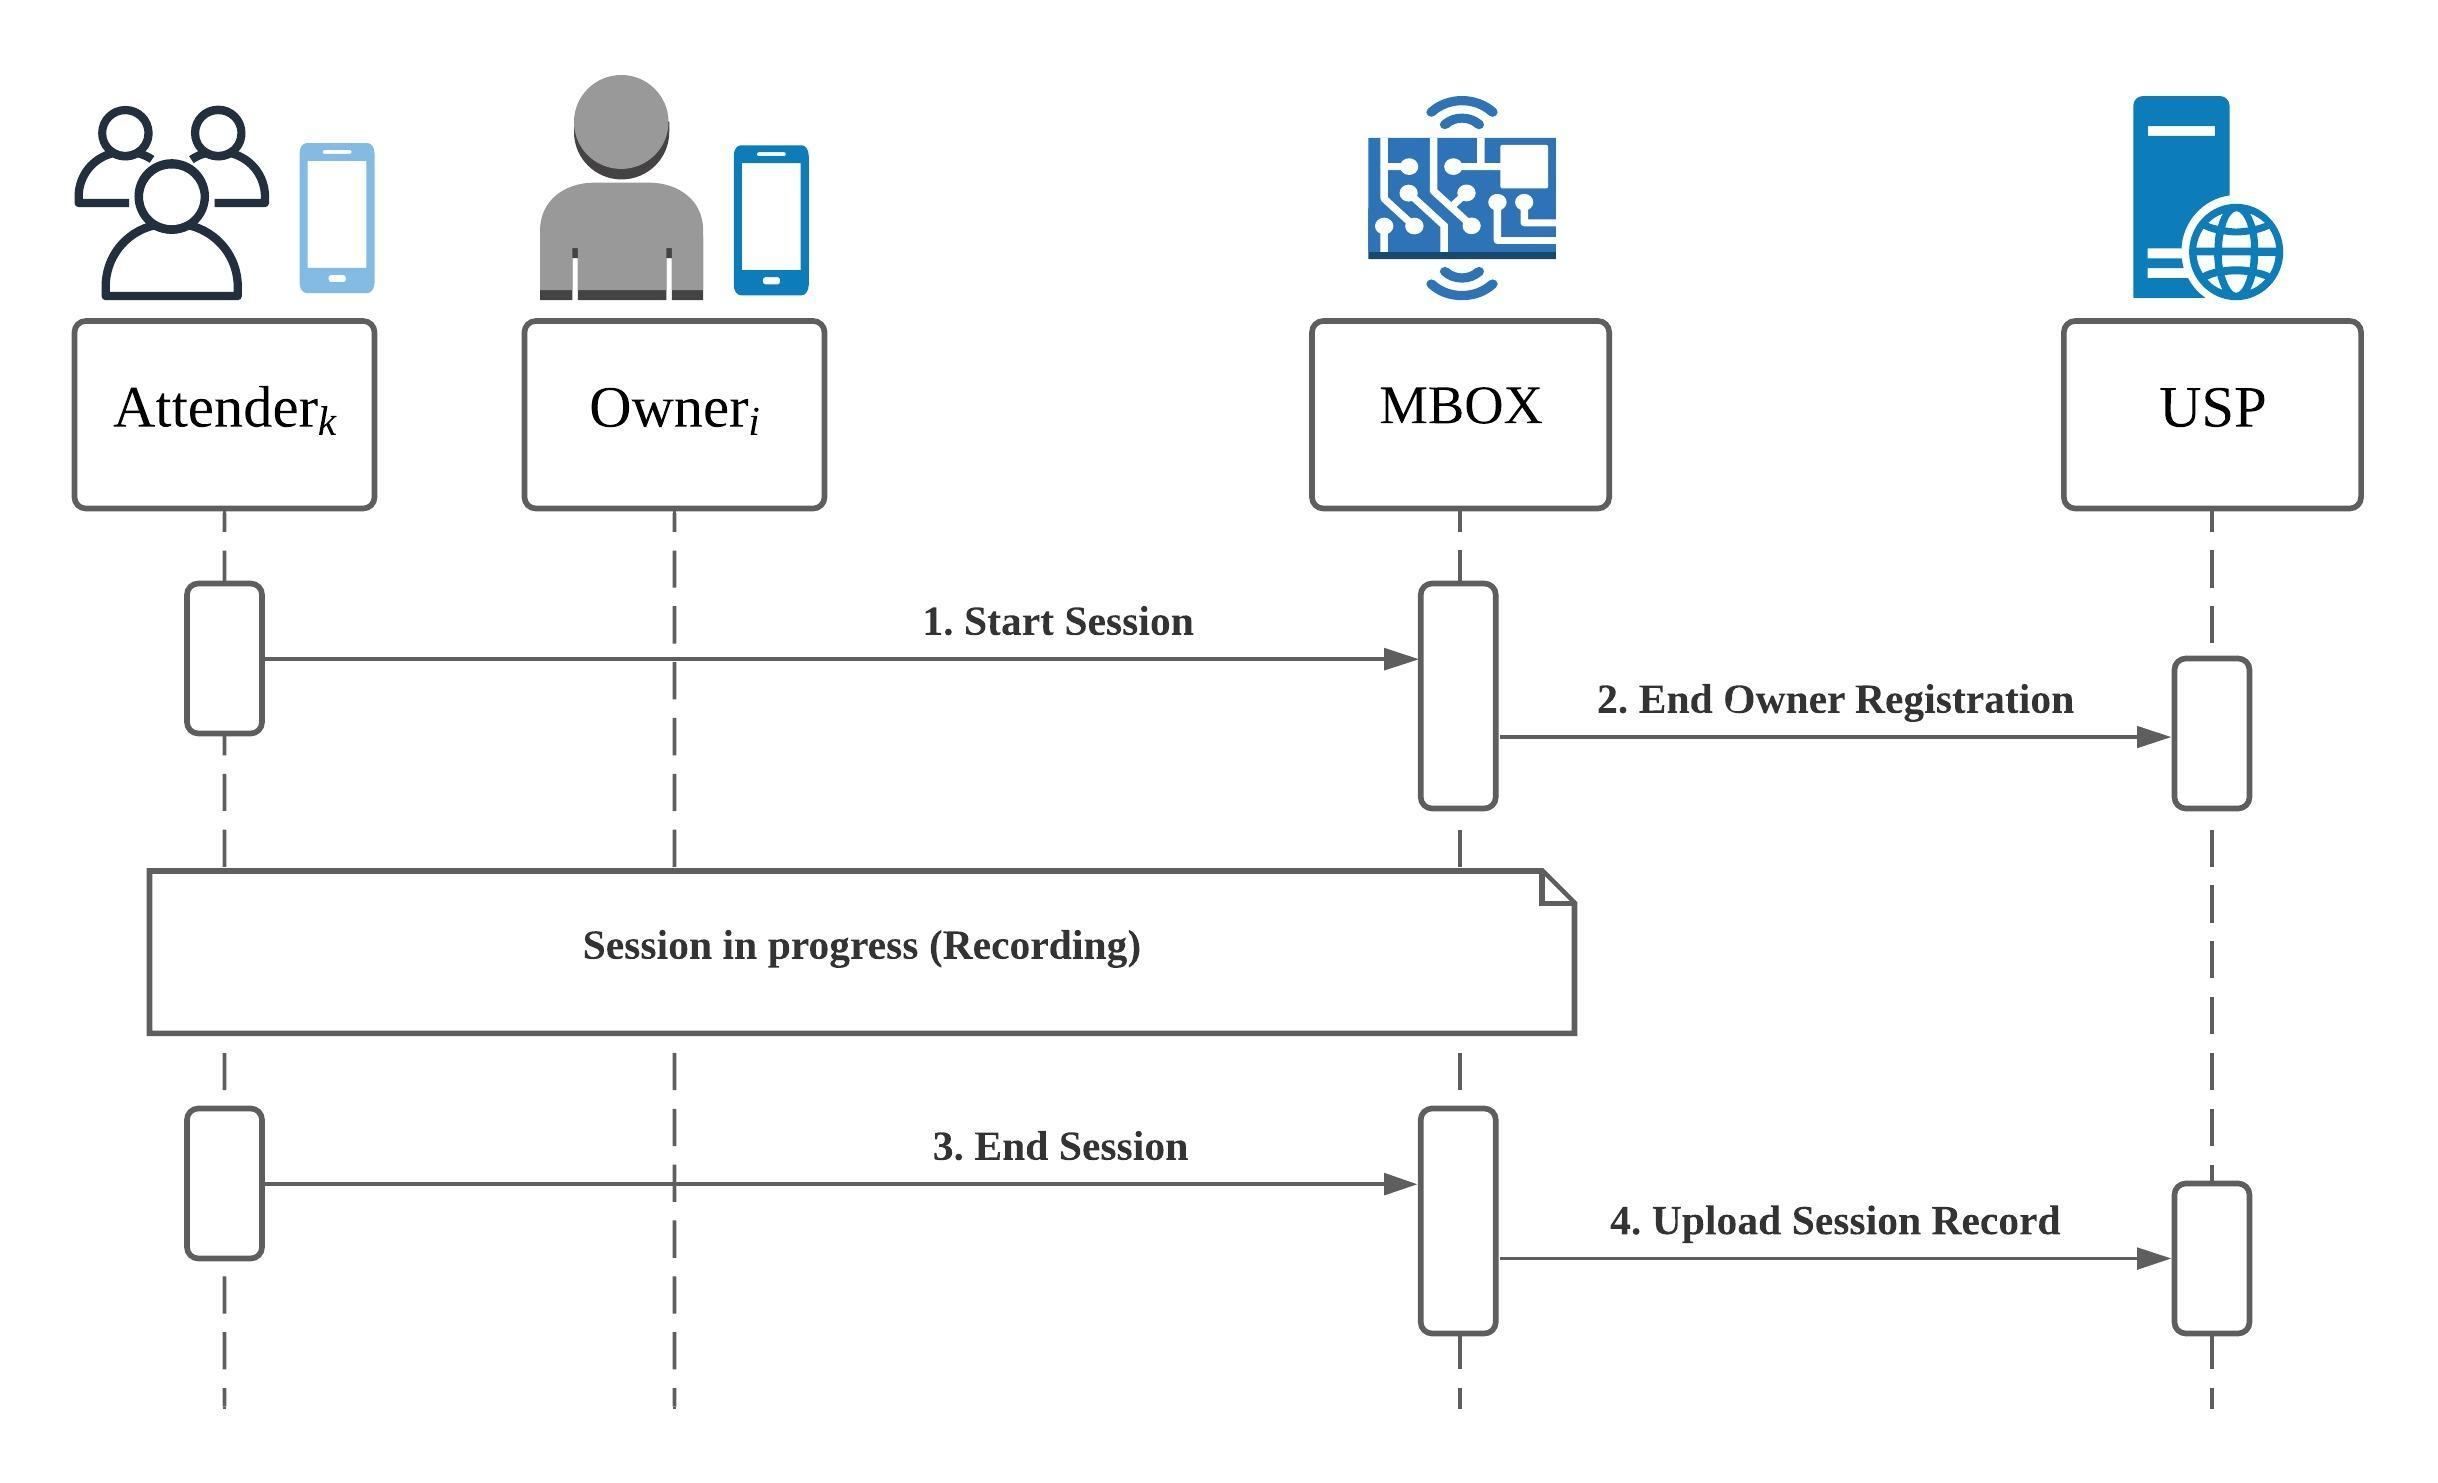
\includegraphics[width=0.9\textwidth]{single-owner-sequence-diagram-sessioning}
    \caption{Single Owner Running {\it Meeting Session}}
    \label{fig.s-o-sessioning}
\end{figure}

\begin{steps}
    \item Start Session (Push Button):

            進入到此階段代表 Owner 已經完成系統機制 Register Owner,MeetingBox 也已初始化完成。
        此時 \DEFattender 即可透過 MeetingBox 的物理控制介面,使 MeetingBox 獲得外部事件,
        觸發 Start Session。

            本研究實驗以按鈕為例,當 \DEFattender 按下 MeetingBox 上的按鈕後,
        觸發 MeetingBox 執行 Start Session。

    \item End Owner Registration:

            MeetingBox 觸發 Start Session 後,接續觸發 Server 執行 End Owner Registration,
        其運作細節如下:一、MeetingBox 對 Server 傳送 End Owner Registration 請求;
        二、Server 透過限制無法在同 \DEFsessionID 綁定新的\DEFprivateKey,
        來終止此 {\it Meeting Session} 註冊產生新的 Owner;
        三、透過 \DEFunsealKey 派生出 \DEFowner 的代理金鑰,定義為 \DEFagentKey。當 \DEFagentKey 產生完即銷毀 \DEFunsealKey 。
        在 {\it Single Owner Meeting Session} 情境中,\DEFagentKey 的值即等於 \DEFunsealKey。
        四、Server 使用此情境中唯一 \DEFowner 的公開金鑰 \DEFpublicKey,透過非對稱式金鑰演算法加密將 \DEFagentKey 加密,
        並銷毀 \DEFagentKey;Server 即完成此系統步驟。

            前述非對稱式金鑰加密演算法,本研究所設計之系統 RSA PKCS \#1 為例。 本文中定義為 \DEFfuncEncPK,
        其輸入為欲加密明文資料,輸出為已加密的密文。加密後的 \DEFagentKey 定義為 \DEFowner 的 \DEFakEnc,
        待 \DEFowner 將其解密方可還原 \DEFagentKey。
        意即,在此情境中,唯一 \DEFowner 的 \DEFakEnc 即為透過 \DEFfuncEncPK 加密的 \DEFunsealKey。

            隨後 MeetingBox 開啟麥克風與超音波麥克風干擾器,並透過 MeetingBox 上的人機互動介面提示系統已經開始錄音。
        麥克風錄製的聲音內容結果 \DEFrecJ,此為超音波麥克風干擾器與會談聲音內容的疊加,屬非有效之聲音記錄。
        此時 Attender 即可進行私密會談,不用擔心有其他麥克風或聲音記錄裝置可以取得有效之聲音記錄。
        前述人機互動介面,本研究實驗以錄音指示燈與螢幕為例,當開始錄音時,將會提示當下系統狀態。

    \item End Session (Push Button):
ㄑ
            當會談對話結束時時 \DEFattender 即可透過 MeetingBox 的物理控制介面,使 MeetingBox 獲得外部事件,
        觸發 End Session。MeetingBox 在此時會關閉麥克風與超音波麥克風干擾器,並產生 \DEFrecJ。
        MeetingBox 上的人機互動介面同時提示系統已結束錄音。

            本研究實驗以按鈕為例,當 \DEFattender 再次按下 MeetingBox 上的按鈕後,
        觸發 MeetingBox 執行 End Session。人機互動介面則以錄音指示燈與螢幕為例,
        當錄音已結束時,前述兩者人機互動介面將會提示當下系統狀態為 End Session。

    \item Upload \DEFrecJ:

            當 Attender 透過 MeetingBox 上的物理控制介面觸發 End Session 後,
        接續觸發 MeetingBox 值行此步驟。此時 MeetingBox 將 End Seesion 步驟結束所產生的 \DEFrecJ,
        上傳至 Server。上傳成功後,即完成進入下一階段。
\end{steps}


\subsection{解封 ({\it Unseal})}
\label{subsec.unseal}

    此章節將說明 {\it Single Owner Meeting Session} 情境中,
{\it Meeting Session} 生命週期第三個階段:{\it Unseal} 的系統流程。
如圖 \ref{fig.s-o-unseal} 所示。此階段執行於 Running {\it Meeting Session} 之後,
Attender 間的談話已結束,Attender 可以離開會談的場域,且不再需要與 MeetingBox 實體接觸。
此階段僅 Owner 與 Server 互動,透過此階段機制,最終可取得有效之會談聲音記錄 (\DEFrecREV)。
本研究所設計之系統可以確保 Server 在 Running {\it Meeting Session}結束後,
直到成功解封 ({\it Unseal})之前,\DEFrecREV 保有機密性。

\begin{figure}[H]
    \centering
    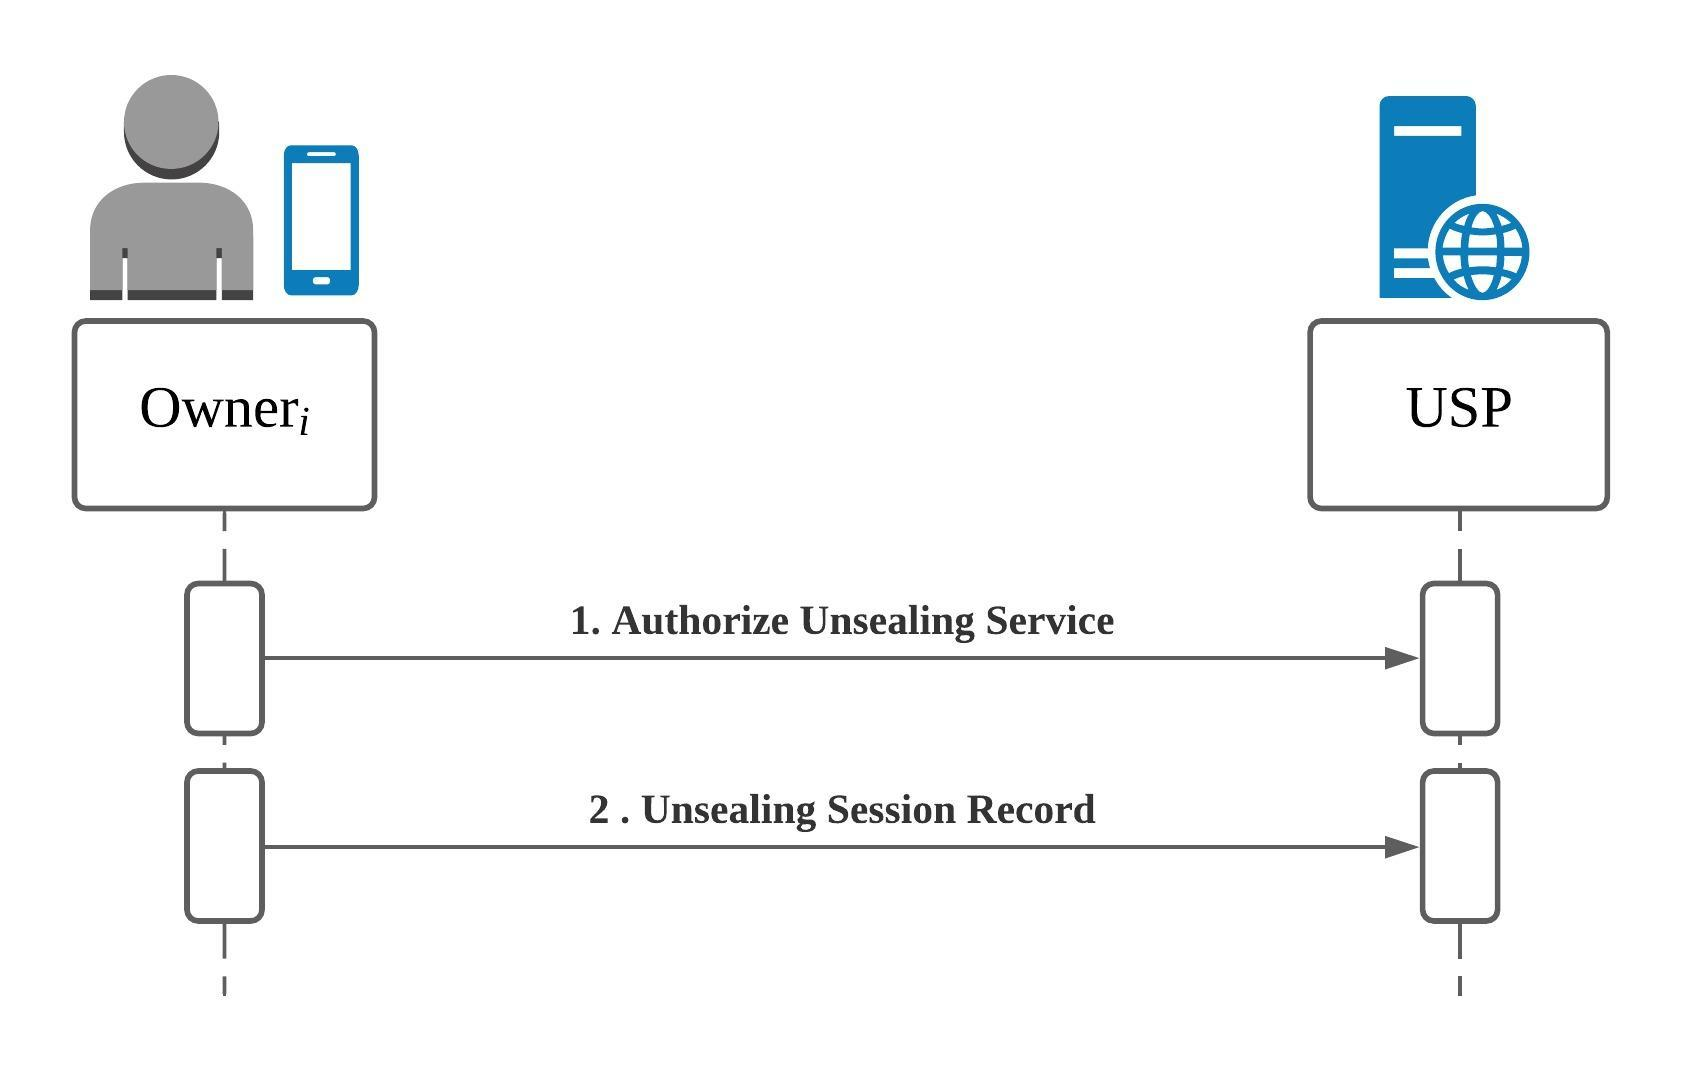
\includegraphics[width=0.7\textwidth]{single-owner-sequence-diagram-unseal}
    \caption{Single Owner {\it Unseal}}
    \label{fig.s-o-unseal}
\end{figure}

\begin{steps}
    \item Unseal Session Record Request:

            在會談對話結束後,Owner 欲取得當時的有效聲音紀錄,則執行此機制。
        \DEFowner 向 Server 傳送 Unseal Session Record Request,
        Server 則回傳 \DEFowner 的 \DEFakEnc。
        {\it Single Owner Meeting Session} 情境中,只有單一個 Owner,
        因此傳送至 \DEFowner 的 \DEFakEnc 其內容,即為使用 \DEFfuncEncPK 加密的 \DEFunsealKey。

    \item Solve Challenge:

            \DEFowner 收到 Server 回傳的 \DEFakEnc 後,因 \DEFowner 持有 \DEFprivateKey,
        因此 \DEFowner 有能力透過相同的非對稱式加密演算法透過其解密。
        而 \DEFakEnc 解密後的明文,本文將其定義為 \DEFakEncDec。

            得到 \DEFakEncDec 後,\DEFowner 再將其透過 \DEFprivateKey 使用數位簽章演算法簽名,
        所產生之簽章,本文定義為 \DEFakEncDecSig。

            \DEFowner 成功產生 \DEFakEncDec 與 \DEFakEncDecSig 後,
        將兩者作為參數向 Server 請求 Solve Challenge。
        Server 收到來自\DEFowner 的 \DEFakEncDec 與 \DEFakEncDecSig 之後,驗證 \DEFakEncDecSig 是否正確。
        透過 Server 的 \DEFpublicKey 利用數位簽章演算法驗證 \DEFakEncDecSig 是否為合法的簽章。
        若簽章合法,依據其不可否認性,Server 得以信任 \DEFakEncDec 的是產生自 \DEFowner。

            於 {\it Single Owner Meeting Session} 情境中,
        \DEFakEnc 的內容為使用 \DEFfuncEncPK 加密的 \DEFunsealKey。
        而 \DEFakEncDec 為解密後的 \DEFakEnc ,即為 \DEFunsealKey,即完成此步驟。
        前述非對稱式金鑰加密演算法,本研究所設計之系統以 RSA PKCS \#1 為例。其解密方法,
        本文定義為 \DEFfuncDecSK,輸入為 \DEFfuncEncPK 輸出的密文,輸出為 \DEFfuncEncPK 的明文輸入。

            前述數位簽章演算法,本研究以 RSA PKCS \#1 與 SHA256 為例。其簽名方法,本文定義為 \DEFfuncSignSK,
        輸入為欲簽名的資料,輸出為資料的簽章。驗證簽章方法,本文定義為 \DEFfuncVerfPK,
        輸入為欲驗證簽名的資料與簽章,輸出為合法與否。

    \item Access Session Record:

            Owner 在前一步驟 Solve Challenge 成功之後,即可再向 Server 發出 Access Session Record 請求。
        若於 Solve Challenge 成功,代表 Server 已獲得此 {\it Meeting Session} 的 \DEFunsealKey。
        此時即可將 \DEFrecN 透過 \DEFunsealKey 輸入對稱式加密演算法的解密函數還原獲得 \DEFrecN。
        前述對稱式加密演算法的解密函數,本研究以 AES CFB mode 為例。本文中定義為 \DEFfuncDecEK,
        其輸入為欲解密的密文資料,輸出解密後的明文。

            Server 上儲存的 \DEFrecJ 為非有效聲音紀錄,其原因為含有高信噪比的噪音。
        此噪音由 MeetingBox 的 超音波麥克風干擾器所產生,與 \DEFrecN 有高相似度與關聯度。
        因此透過 \DEFrecN 與 \DEFrecJ 輸入 「主動式噪音控制」(ANC),即可獲得有效會談聲音記錄。
        透過 ANC 還原的有效會談聲音記錄,本文定義為 \DEFrecREV。
\end{steps}


\subsection{{\it Multi Owner Meeting Session}}

此章節將說明 Multi Owner Meeting Session 情境中,系統生命週期階段的流程步驟。
當存在 {\it Meeting Session} 中 Owner 數量為二人以上,即定義為 Multi Owner Meeting Session 之情境。
於此情境中,{\it Meeting Session} 生命週期的三個階段與前篇 Single Owner Meeting Session 情境相似。
其差異之處在於 Owner 數量大於二人。基於前篇 Single Owner Meeting Session 情境,
僅需小幅度的系統改動與引入 Shamir's Secret Sharing,即可達成 Multi Owner Meeting Session 情境。

\begin{figure}[H]
    \centering
    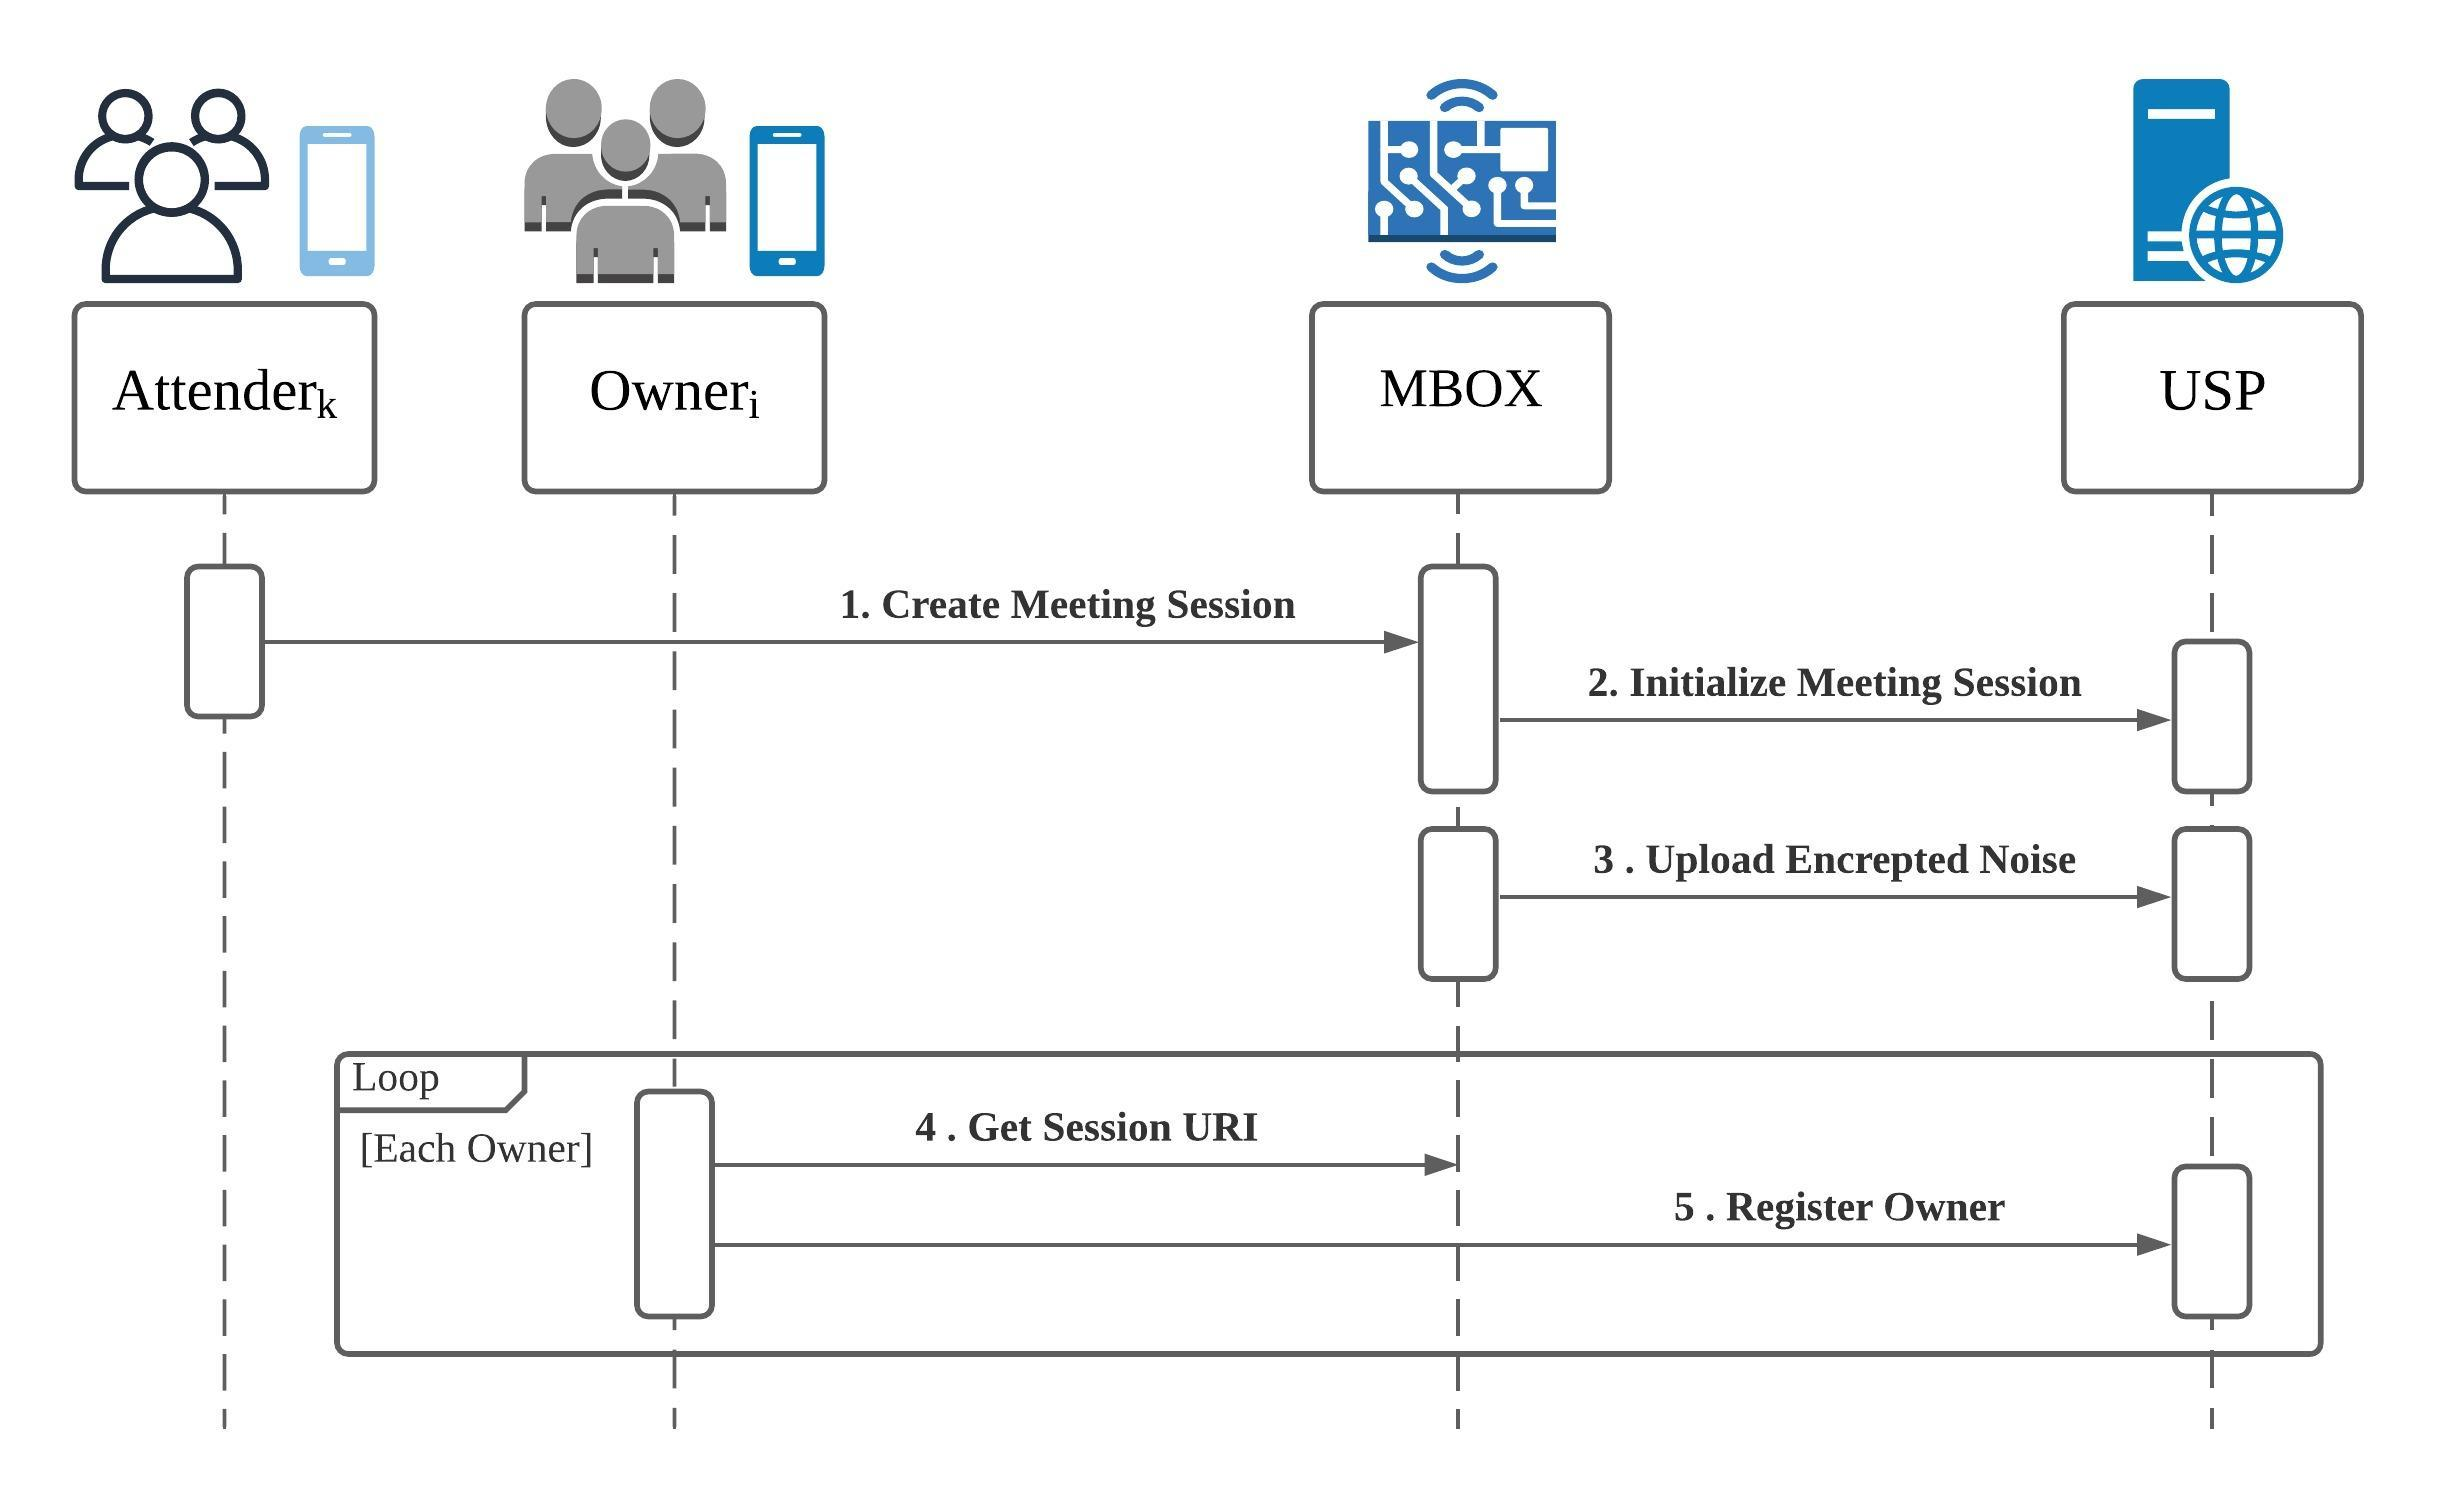
\includegraphics[width=0.9\textwidth]{multi-owner-sequence-diagram-init}
    \caption{Multi Owner Initialize {\it Meeting Session}}
    \label{fig.m-o-init}
\end{figure}

    {\it Multi Owner Meeting Session} 情境中,
{\it Meeting Session} 生命週期第一個階段:Initialize {\it Meeting Session} 的系統流程。
如圖 \ref{fig.s-o-init} 所示。

\begin{figure}[H]
    \centering
    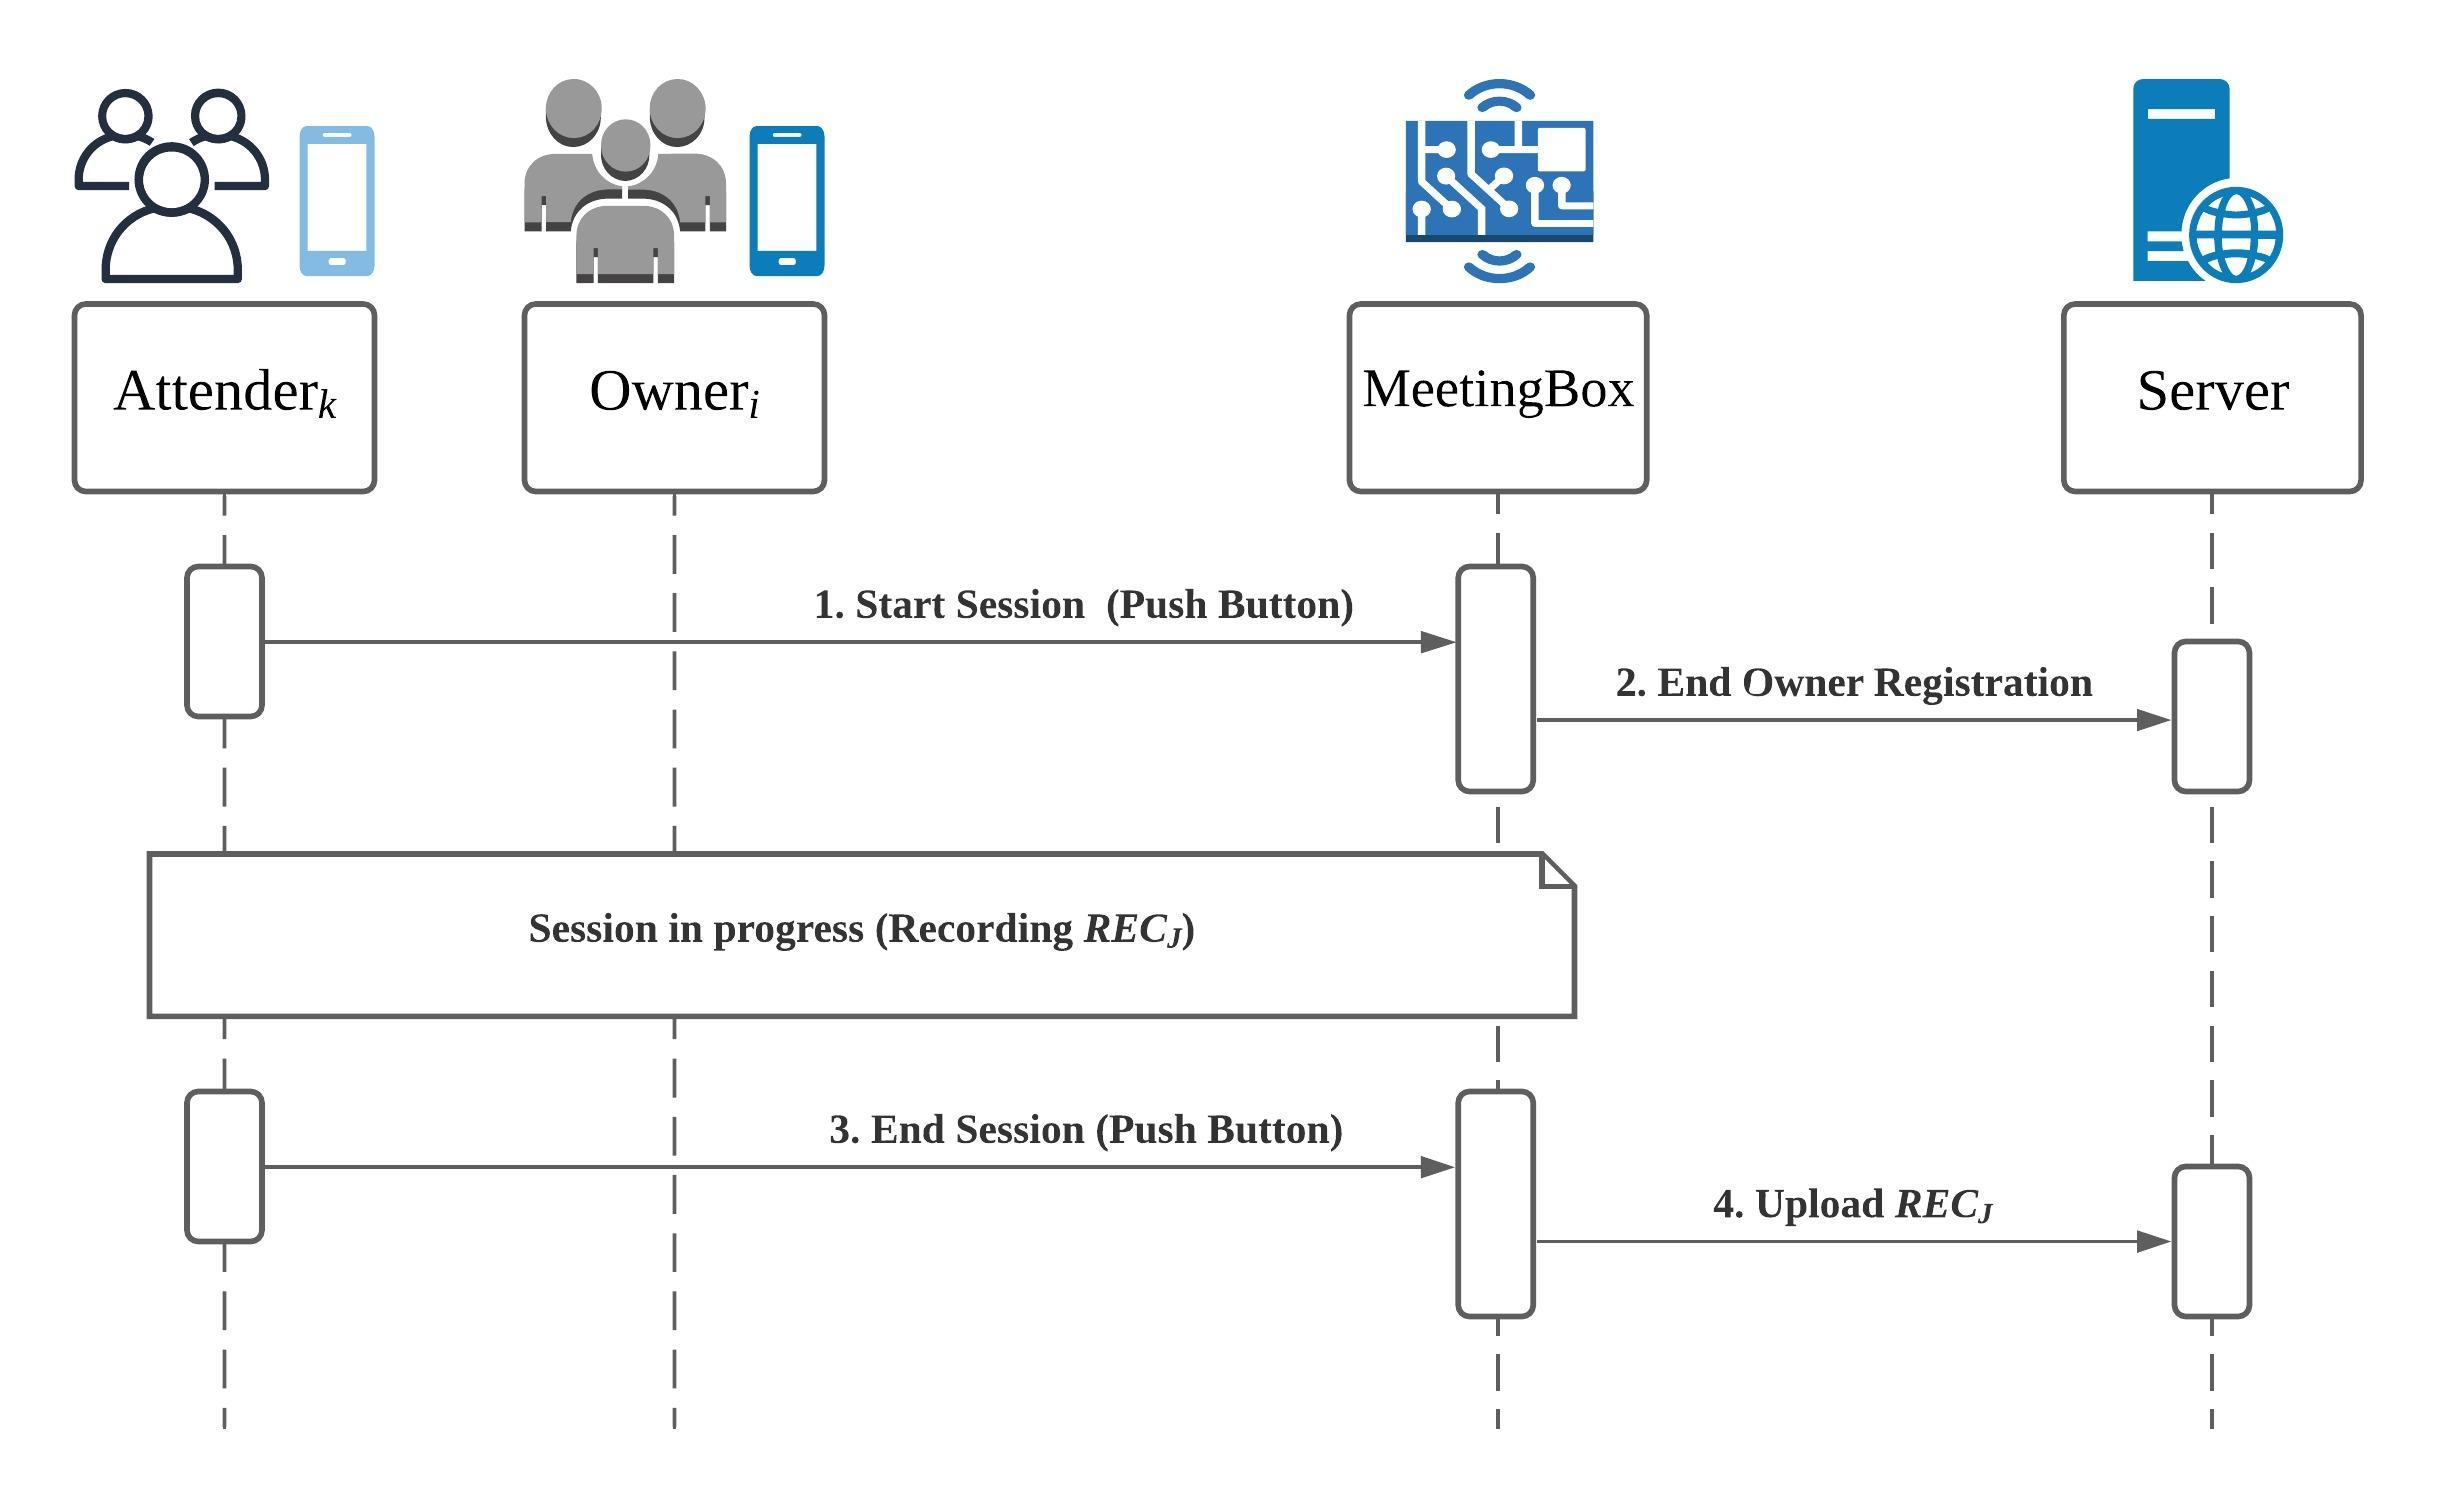
\includegraphics[width=0.9\textwidth]{multi-owner-sequence-diagram-sessioning}
    \caption{Multi Owner Running {\it Meeting Session}}
    \label{fig.m-o-sessioning}
\end{figure}

\begin{figure}[H]
    \centering
    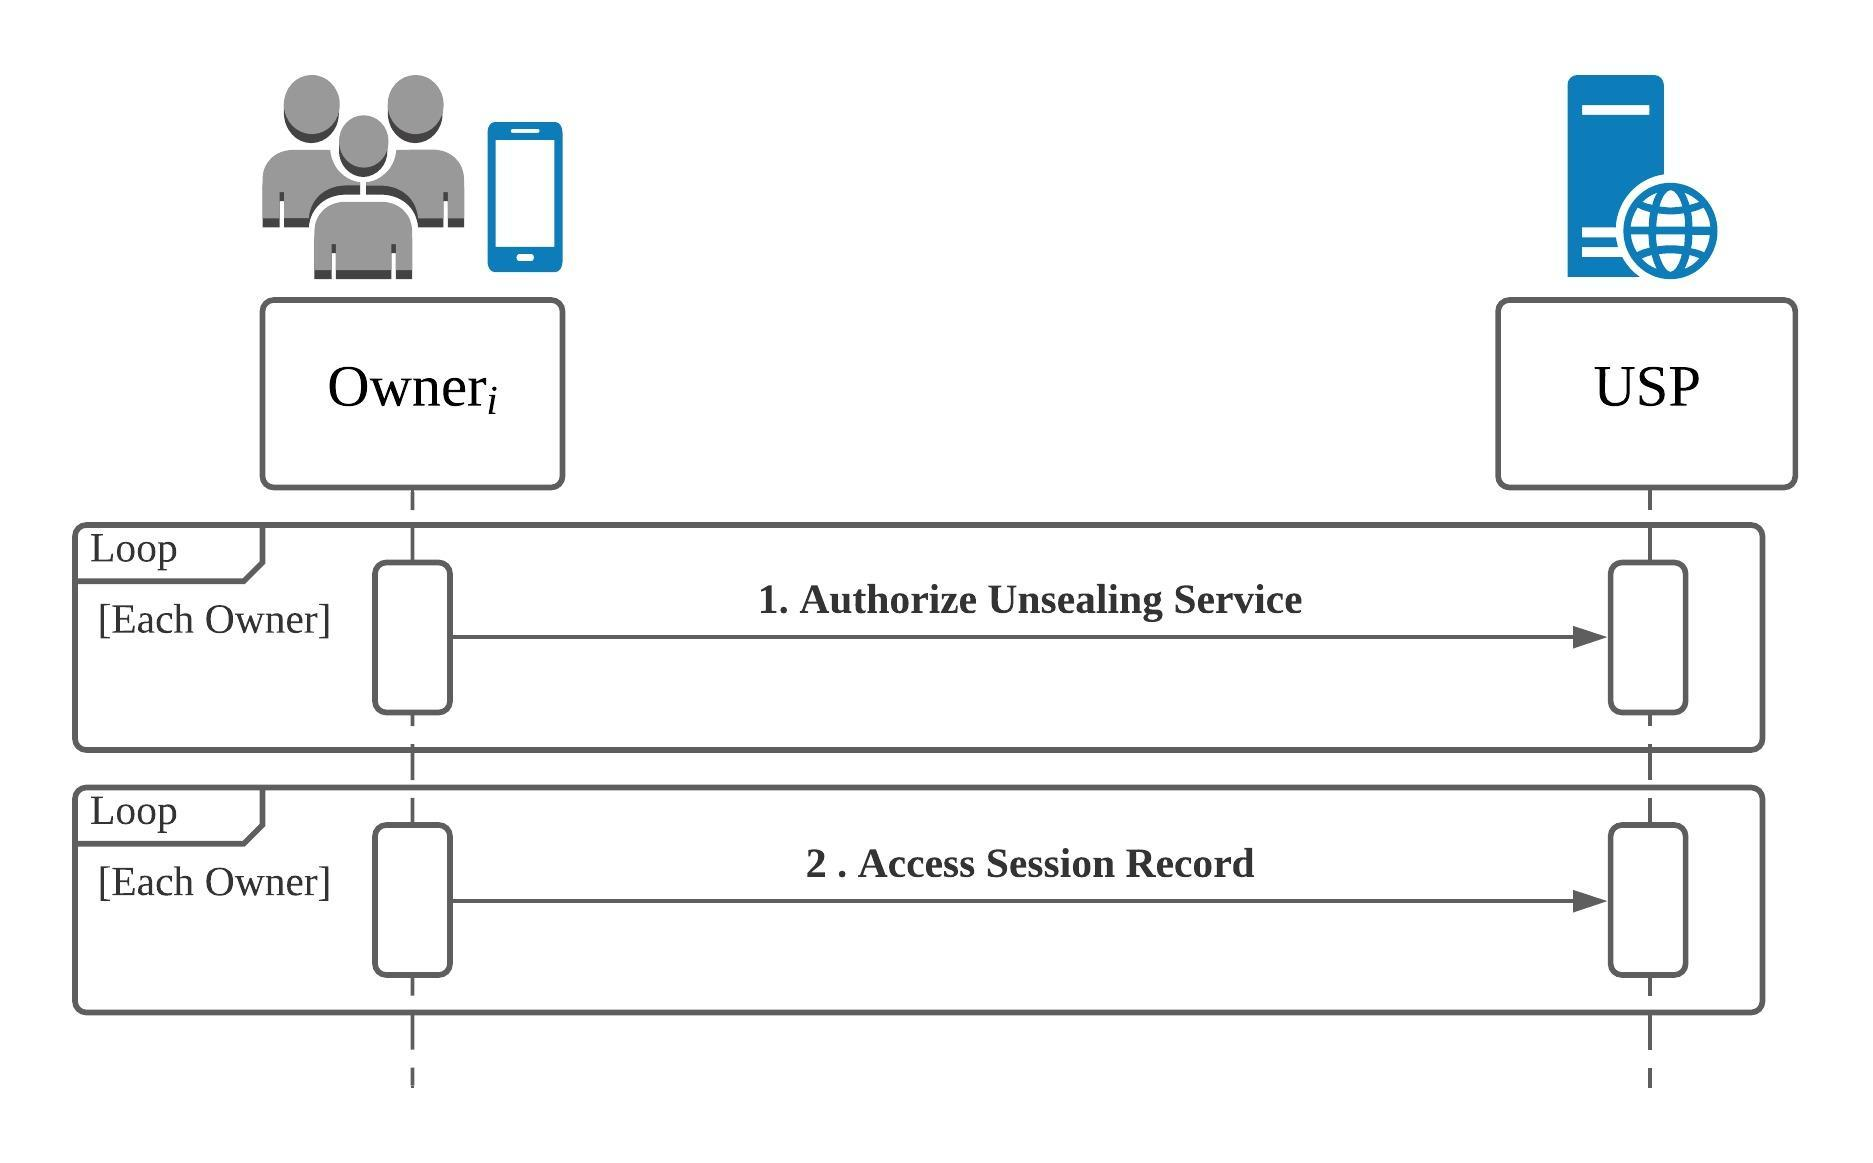
\includegraphics[width=0.7\textwidth]{multi-owner-sequence-diagram-unseal}
    \caption{Multi Owner {\it Unseal}}
    \label{fig.m-o-unseal}
\end{figure}


\section{系統機制}

\subsection{錄音存取控制與解密}

\begin{center}
\noindent
\begin{tabularx}{0.95\textwidth} {
        |c
        >{\raggedright\arraybackslash}X
        >{\centering\arraybackslash}c
        >{\raggedright\arraybackslash}X
        c|
    }
    \hline

    & \multicolumn{1}{c}{\bf{Meetingbox}} &
    & \multicolumn{1}{c}{\bf{Server}} & \\

    & \multicolumn{1}{c}{$\{\}$} &
    & \multicolumn{1}{c}{$\{\}$} & \\

    \cline{2-2} \cline{4-4}

    &
    pseudocode
    & & & \\

    & &
    $\xrightarrow{~~M~~}$
    & & \\

    & & &
    pseudocode
    & \\

    \hline
\end{tabularx}
\end{center}


\subsection{主動式噪音控制}

\subsection{樣本對齊}

\section{系統實作}